
\subsection{Subsystem 1 camera subsystem}
This section should be a general description of a particular subsystem for the given layer. For most subsystems, an extract of the architectural block diagram with data flows is useful. This should consist of the subsystem being described and those subsystems with which it communicates.

\begin{figure}[h!]
	\centering
 	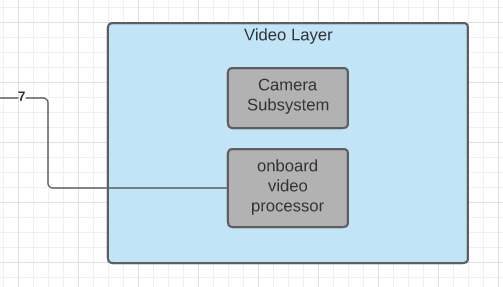
\includegraphics[width=0.60\textwidth]{images/subsystem_video}
 \caption{Example subsystem description diagram}
\end{figure}

\subsubsection{Assumptions}
We made the assumption that we would not be able to navigate the submarine without an underwater perspective.

\subsubsection{Responsibilities}
the responsibility of the camera is to capture the perspective of the submarine and relay it back to the video monitor.

\subsubsection{Subsystem Interfaces}
Each of the inputs and outputs for the subsystem are defined here. Create a table with an entry for each labelled interface that connects to this subsystem. For each entry, describe any incoming and outgoing data elements will pass through this interface.

\begin {table}[H]
\caption {Subsystem interfaces} 
\begin{center}
    \begin{tabular}{ | p{1cm} | p{6cm} | p{3cm} | p{3cm} |}
    \hline
    ID & Description & Inputs & Outputs \\ \hline
    \#xx & USB interface & \pbox{3cm}{USB } & \pbox{3cm}{USB port to Raspberri pi}  \\ \hline
    \end{tabular}
\end{center}
\end{table}

\subsection{Subsystem 2 onbaord video processor} 
\subsubsection{Assumptions}
We made the assumption that we the video will need to be relayed to some sort of small computer for processing and then sending on its way to our video monitor system.

\subsubsection{Responsibilities}
take the live USB feed of the video camera and propagate it back to our video monitor via the tether.

\subsubsection{Subsystem Interfaces}
\begin {table}[H]
\caption {Subsystem interfaces} 
\begin{center}
	\begin{tabular}{ | p{1cm} | p{6cm} | p{3cm} | p{3cm} |}
		\hline
		ID & Description & Inputs & Outputs \\ \hline
		\#xx & USB interface & \pbox{3cm}{USB } & \pbox{3cm}{Tether wire}  \\ \hline
	\end{tabular}
\end{center}
\end{table}


